
\section{Numerical simulations for indirect file piece loss}
\subsection{Introduction}
We produce decision tables showcasing worst-case mean file rebuild outcomes based on simulating file piece loss for files encoded with varying Reed-Solomon parameters.
We assume an $(k,n)$ RS encoding scheme, where $n$ pieces are generated, with
$k$ pieces needed for reconstruction, using three different values for $n$.
We assume that a file undergoes the process of repair when less than $r$ pieces remain on the network, using three different values of $m$ for each $n$.
For the initial table, we use a simplifying assumption that pieces on the network are lost at a constant rate per month\footnote{This constant rate may be viewed as the mean of the Poisson distribution modeling piece loss per month.}, which may be due to node churn, data corruption, or other problems.


To arrive at the value for mean rebuilds per month, we consider a single file that is encoded with $n$ pieces which are distributed uniformly randomly to nodes on the network. To simulate conditions leading to a rebuild, we uniformly randomly select a subset of nodes from the total population and designate them as failed. We do this multiple times per (simulated) month, scaling the piece loss rate linearly according to the number of file integrity checks (``checks'') per month\footnote{
For example, if the monthly network piece loss rate is assumed to be 0.1 of the network size (or 10\%), and if 10 file integrity checks are performed per month, we assume that, on average, 1\% of pieces are lost between checks.}.
Once enough nodes have failed to bring the number of file pieces under the repair threshold, the file is rebuilt, and we track the number of rebuilds over the course of 24 months.
We repeat this simulation for 1000 iterations, simulating 1000 2-year periods for a single file. We then take the number of rebuilds at the 99-th percentile (or higher) of the number of rebuilds occurring over these 1000 iterations. In other words, we choose the value for which the value of the observed cumulative distribution function (CDF), describing the number of rebuilds over this 2 year period, is at least 0.99. This value is then divided by the number of months to arrive at the mean rebuilds/month value. An example of the approach is shown in Figure \ref{fig:sim_method}. We perform the experiment on a network of 10,000 nodes, observing that the network size will not directly impact the mean rebuilds/month value for a single file under our working assumption of a constant rate of loss per month\footnote{We represent piece loss as a proportion of nodes selected uniformly randomly from the total network. The proportion scales directly with network size, so the overall number of pieces lost stays the same for networks of different sizes.}.

\linespread{1}
\begin{figure}[h]
    \centering
    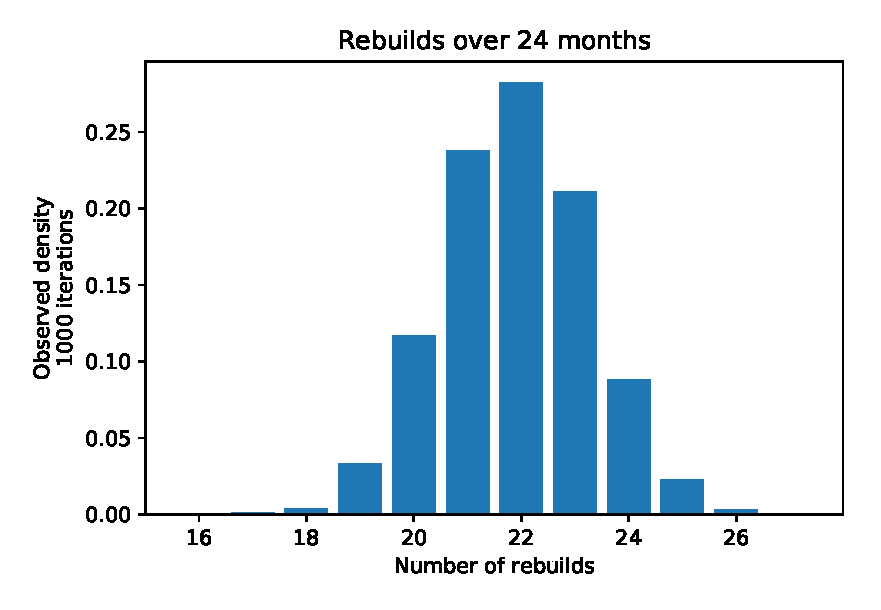
\includegraphics[scale=0.5]{RS-appendix-files/example_pmf.eps}
    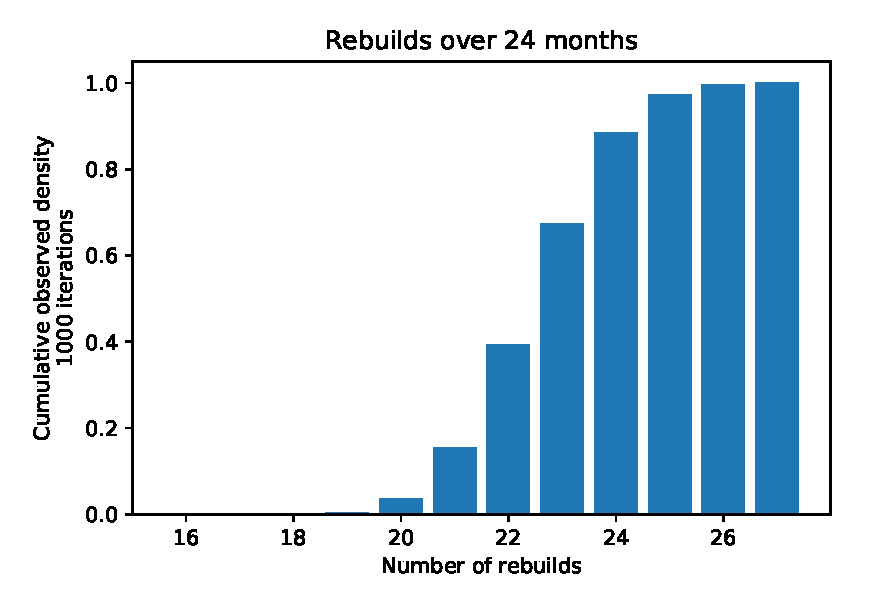
\includegraphics[scale=0.5]{RS-appendix-files/example_cdf.eps}
    \caption{Top: Density for the number of rebuilds over a 24 month period, repeated for 1000 iterations. Bottom: CDF of the number of rebuilds. In this case, the mean rebuilds/month value would be taken as $26/24\approx1.083$, with there being a 99.7\% chance that a file is rebuilt at most 26 times over the course of 24 months.}
    \label{fig:sim_method}
\end{figure}

\pagebreak
\linespread{1}
\pagebreak
\subsection{The decision tables}
In forming the decision tables, we consider as part of our calculations how
different choices of $k$, $n$, $m$, and mean time to failure affect durability and repair bandwidth. What we are looking for is the lowest repair bandwidth that also meets our
durability requirements.
\begin{table}[!htpb]\centering

\begin{tabular}{| c | c c c | c | c|}\hline
MTTF (months) &$k$& $n$ & $m$ &Repair Bandwidth Ratio&Durability (\# nines) \\\hline
1 &20& 40 & 35 & 9.36 & 0.9999 (8) \\
6 &20& 40 & 30 & 0.87 & 0.9999 (17) \\
12 &20& 40 & 25 & 0.31 & 0.9999 (13)\\\hline

1 &30& 60 & 35 & 3.40 &0.9999 (4)\\
6 &30& 70 & 40 & 0.60 &0.9999 (15)\\
12 &30& 80 & 45 & 0.31 &0.9999 (25) \\\hline

1 &40& 80 & 60 & 5.21 &0.9999 (4)\\
6 &40&120&50 & 0.52 &0.9999(14)\\
12 &40&120&45 & 0.24 &0.9999 (11)\\\hline

\end{tabular}
\caption{Decision tables showing the relationship between churn (MTTF),
  Reed-Solomon parameters ($k$, $n$, $m$), repair bandwidth ratio, and durability}
\label{rs:decision-tables}
\end{table}



